\chapter{sPHENIX Commissioning}
\label{chap:commissioning}

As expected with any new collider detector, there will be significant
commissioning time required in order to be ready for physics quality
data.  The sPHENIX project and collaboration teams have taken this
task seriously with detailed input from the detector subsystems and
the sPHENIX Physics Working Groups.  We detail the initial
commissioning plan and timeline for 2023 in this Chapter.   

\section{2023 \auau Commissioning Timeline}

\renewcommand{\arraystretch}{1.9}
\addtolength{\tabcolsep}{-0.5pt}
\begin{table}[]
  \caption{\label{tab:commision}Timeline for sPHENIX commissioning
    period in 2023, the first year of operation.}
    \centering
    \begin{tabular}{S[table-format=2.1]l} \toprule
        {Weeks} &  Details \\ \midrule
        1.5 & low rate, 6 bunches \\ 
        2.0 & low rate, 111 bunches, MBD L1 timing \\ 
        1.0 & low rate, crossing angle checks \\ 
        1.0 & low rate, calorimeter timing \\ 
        4.0 & medium rate, TPC timing, optimization \\
        2.0 & full rate, system test, DAQ throughput \\ \bottomrule
        11.5 & {\bf total} 
    \end{tabular}
\end{table}

Commissioning sPHENIX with beams in RHIC should progress in stages
with gradually increasing luminosity.  \auau collisions are necessary
for commissioning due to the high multiplicities which can be used to
assess the detector performance with larger occupancy.  We note that
installation of the sPHENIX inner silicon detectors takes 2--3 weeks
and thus these sensitive detectors will be installed ahead of the 2023
running period for system debugging and cosmic ray data taking.  The
presence of the full detector configuration means that very careful
monitoring of luminosity and beam conditions is essential to maintain
stable operations and minimize detector risk.  Thus, the sPHENIX
experiment will require very careful coordination with C-AD including
potential accelerator down times for access.  A summary of the
projected initial commissioning timeline is shown in
Table~\ref{tab:commision}.

%\section{Commissioning Period Details}

For the purposes of this Beam Use Proposal, we include a very brief
summary of the timeline as given.  Except for initial stores with six
bunches, operation with the maximum number of bunches (111) is
preferable to reducing luminosity by reducing the number of filled
bunches because it allows sPHENIX to commission as it plans to run.
Initial stores should be zero crossing angle, both to begin operations
with stores less likely to be lost as well as to provide a direct
comparison of vertex distribution between crossing angles of zero and
the nominal 2 milliradians.

The superconducting solenoid should be operating at full field during
the commissioning.  The minimum bias detector (MBD) gains are reduced
by the magnetic field, and so tuning should take place at the field
planned for physics operation.

\begin{itemize}

\item Initial studies will require 1.5 weeks of stores with six
  bunches, zero crossing angle, and a collision rate of up to 2~kHz.
  These collisions will be used for an initial tune-up of timing and
  the MBD trigger.  A simple ''blue logic'' trigger may be used
  initially for timing.  Several days may be required before we can
  fully operate the detector to provide time for use of diagnostic
  instrumentation and to process data, but the stores can be kept in
  RHIC as long as practical.

\item The next period will consist of two weeks of stores with 111
  bunches, zero crossing angle, and a collision rate of 1--5~kHz.
  These stores will be used for optimizing the MBD Level-1 (L1)
  trigger, which may require additional timing adjustments of the
  trigger primitives.  This phase will also require relatively short
  periods of data taking followed by analysis and diagnostics.  Near
  the end of this period, the calorimeters could be turned on, and
  timing them in could be attempted if it was not already done during
  the previous period.  Operation during the second week will employ
  the planned crossing angle.  This should allow the first measurement
  of the vertex distribution with the planned crossing angle and
  begin any optimization of the ramp that may be necessary while the
  tracking detectors, including the two inner silicon detectors, are
  turned off.

\item We estimate that it will take a week of machine studies at this
  point to optimize the beam crossing angle.  Careful coordination
  between sPHENIX and RHIC operations will be important in this stage.

\item The next week will consist of stores with 111 bunches and
  non-zero crossing angle, and will be used for calorimeter timing and
  tuneup.  The crossing angle will allow us to assess the radiation
  dosage to the silicon photo-multipliers (SiPMs) by measuring the
  leakage current with the monitoring system.

\item The next phase will consist of four weeks of stores with 111
  bunches, non-zero crossing angle, and a collision rate of 1--5 kHz.
  These stores will be used for initial operation of the tracking
  detectors, beginning with the TPC.  The minimum bias trigger,
  developed in the previous weeks, will be used to trigger the
  detector.  It may be useful during this phase to operate with zero
  magnetic field and/or very low luminosity for periods of time in
  order to collect data which can be used to align the tracking
  detectors and characterize track distortions.  Some additional time
  may be necessary for data taking at zero field in order to change
  the MBD high voltage for zero field.

\item The next two weeks will involve stores with 111 bunches,
  non-zero crossing angle, and an increasing rate of minimum bias
  collisions, culminating in fills that provide 15--20~kHz of
  collisions in order to stress test the data acquisition system under
  target running conditions.

\end{itemize}

At the end of this 11.5 week commissioning plan, the detector should be
ready to take data from all detectors, triggered according to plan for
\auau, at the design rate of the data acquisition system.  Of course,
producing data of publication quality requires more analysis than can
be brought to bear while the collaboration is commissioning the
apparatus, so it is crucial to develop monitoring software which
allows us to quickly assess the quality of data as we take it.  We
note that such commissioning time always has a significant uncertainty,
and run time flexibility in this first year of running will be
required.

Additional trigger specific commissioning time is needed for each new
collision species, particularly the physics-selective Level-1 triggers
in the 2024 \pp and \pau running.  This commissioning time is built
into the ramp up calculation for integrated luminosities in these
periods.  We highlight that we have also included a 60\% up-time for
the sPHENIX detector in 2023 and 2024, and then an 80\% up-time in
2025.

\section{2023 \pp Commissioning Option}
\label{sec:year1pp}

There is a definite benefit if sPHENIX would have an opportunity to start commissioning beam conditions, triggering, and detector setup for \pp collisions at 200 GeV in Year-1 (2023) of running.   
With the commissioning plan for \auau detailed in Section~\ref{sec:auaucomm}, which takes precedence to make sure sPHENIX operates up to specifications in the highest multiplicity environments, and only 24 or 28 cryo-weeks in Year-1, 
the plan currently precludes running \pp in the same run.    However, if the sPHENIX commissioning were to go faster than expected with positive results and / or additional cryo-weeks might be available, a minimum running time of
6-7 cryo-weeks for unpolarized \pp running would be beneficial ahead of the planned Year-2 (2024).   Having this commissioning run as unpolarized will enable C-AD to potentially shorten the setup time and focus on critical beam conditions.

Again, \auau running is the highest priority for commissioning, but 6-7 additional 
cryo-weeks  for \pp running could be used for trigger development, a first look at the detector with low-multiplicity events, and potentially collect a sample of triggered photon data which could be used to characterize the jet energy scale (JES) using photon-jet
events.   This run would be a test of the detector and RHIC operation in advance of
the longer \pp run planned for Year-2 (2024). 

\begin{table}[]
    \centering
    \begin{tabular}{|c|l|} \hline
        Weeks & Designation \\ \hline
        1.0-2.0 & Set-up mode 2 (\pp at 200 GeV)  \\ \hline
        1.0    & Ramp-up mode 2 (work to design luminosity with non-zero crossing) \\ \hline
        2.0   & Timing and trigger development \\ \hline
        2.0.  & Data taking mode 2 (Physics) \\ \hline \hline
        6.0-7.0 & Total cryo-weeks \\ \hline
    \end{tabular}
    \caption{Potential commissioning and short data taking schedule for \pp 200 GeV running in Year-1.}
    \label{tab:pp1schedule}
\end{table}

Two weeks of data taking could potentially provide 10-15~\pb of triggered photon
\pp data with a non-zero crossing angle which would allow a first attempt 
at determining the jet energy scale in \pp collisions with the sPHENIX detector.
We note that even 15~\pb of collected, triggered photon data would give a 1.5\%
JES uncertainty in the ``golden channel'' photon-jet balance at 20 GeV as shown in Figure~\ref{fig:jes}.   Such an initial commissioning and check on the JES in \pp collisions would be beneficially entering the long \pp running in Year-2, as well as very useful in fully understanding the Year-1 \auau data set.

\begin{figure}
    \centering
    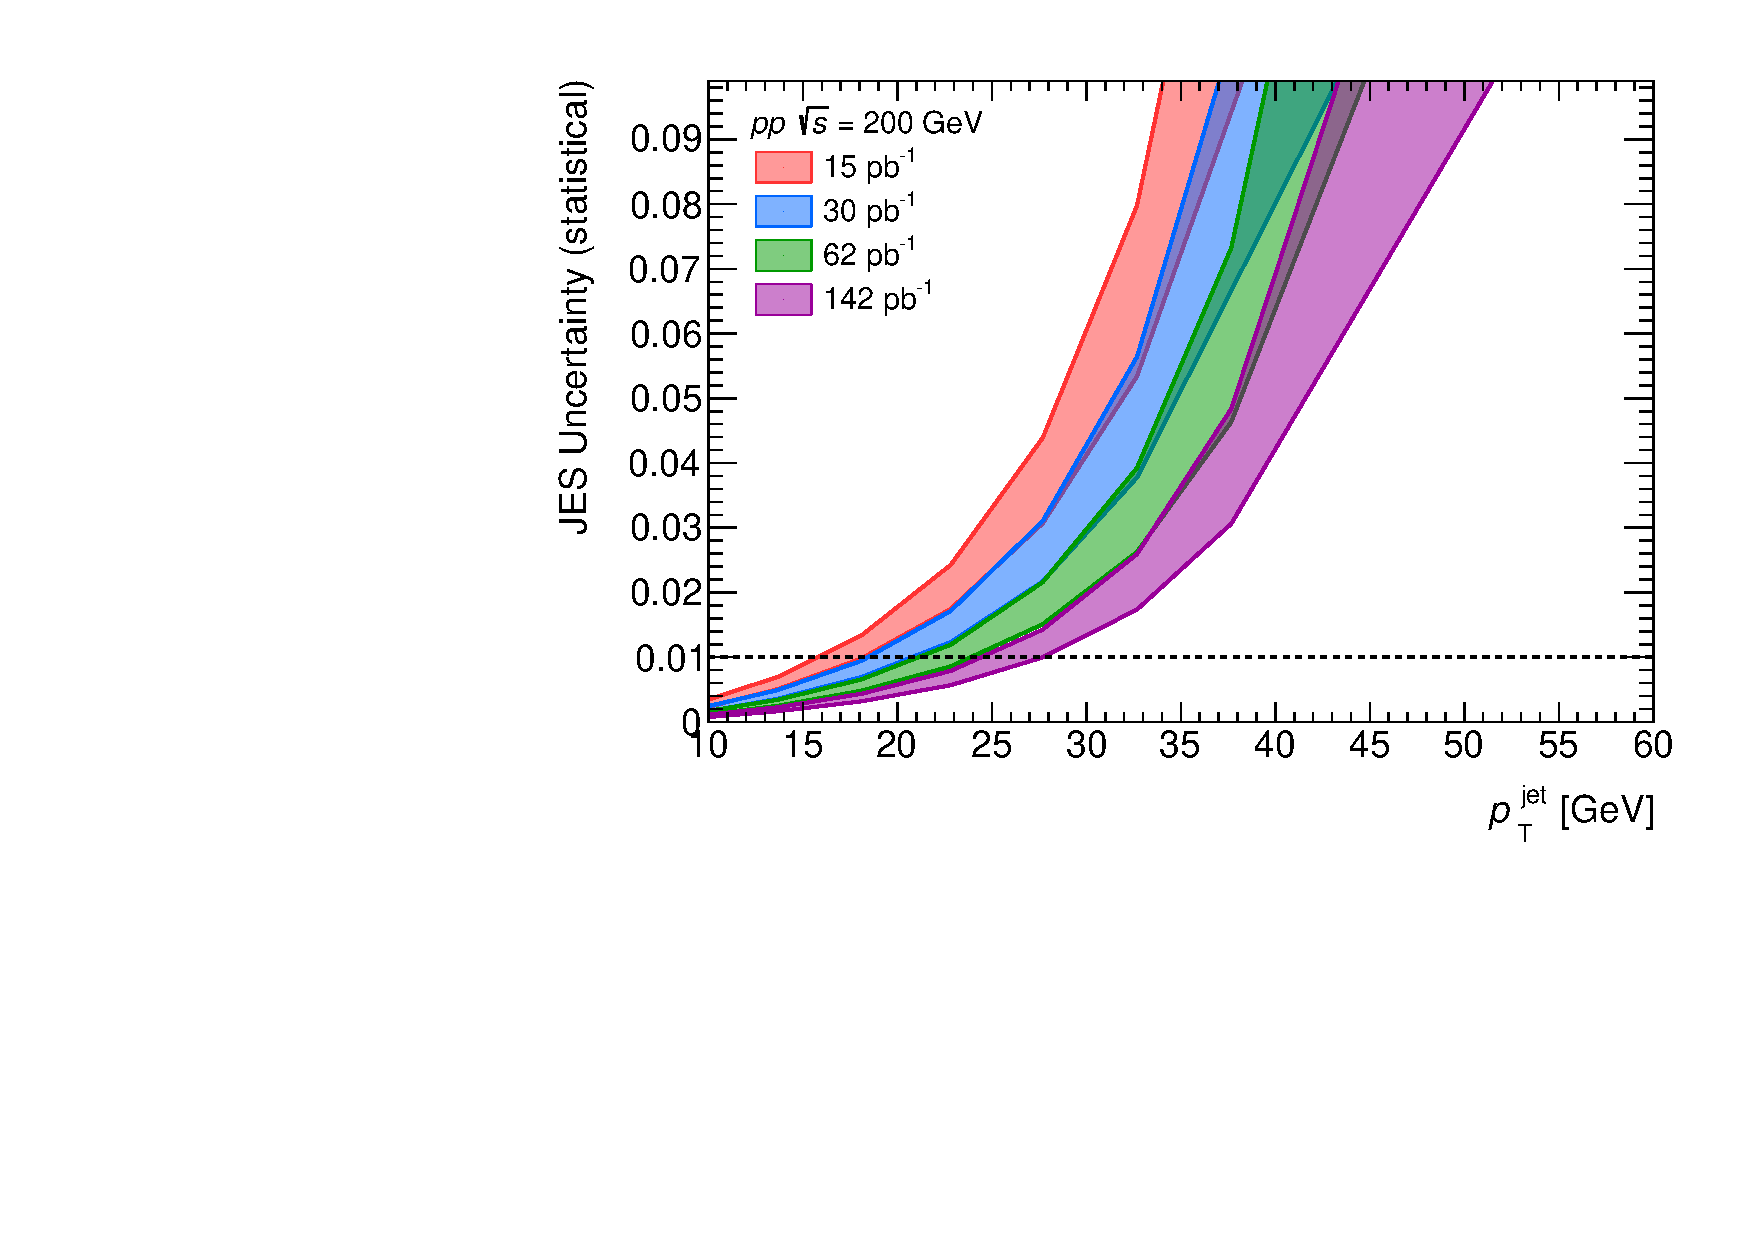
\includegraphics[width=0.8\linewidth]{figs/CompareSqrtsBUR.pdf}
    \caption{The projected sPHENIX statistical uncertainty contribution to the Jet Energy Scale (JES) uncertainty as determined from the ``golden channel'' via photon-jet direct balance studies.  The dashed line at 1\% represents a final JES uncertainty goal.}
    \label{fig:jes}
\end{figure}

